\section{Control Sequences} \label{sec:sequences}
By setting the control signals as described in Section \ref{sec:architecture} appropriately, the modules can work together to perform each of the BF instructions. Table \ref{tab:microcode} shows the control sequences that are executed per BF instruction (also known as microcode instructions). The Control Unit implements this as a lookup table in ROM, where the instruction (in I), flags (also in I) and cycle counter (kept by the CU) act as an address into this table and the control signal configuration is stored at this address in ROM (Figure \ref{fig:decoder}).

\begin{figure}[H]
  \centering
  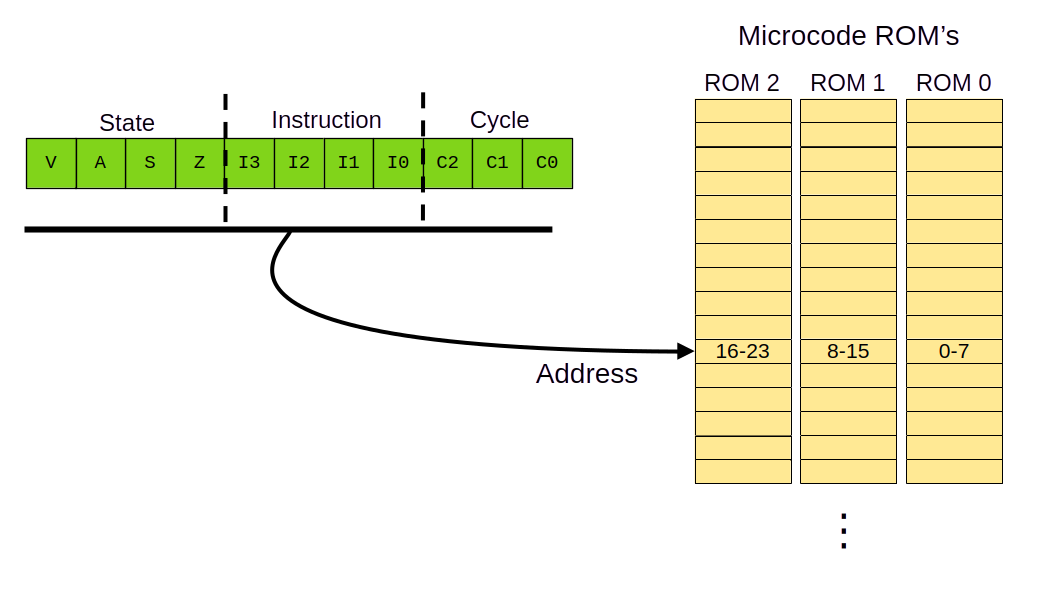
\includegraphics[width=0.9\textwidth]{img/instruction_decoding}
  \caption{Decoding an instruction: the current instruction and state index the ROM, which returns the control signal configuration.}
  \label{fig:decoder}
\end{figure}

It is important to note that, because of the choice of driving all of the (counting) registers with a common interface (Section \ref{sec:implementation:registers}), only one register can be driven each clock cycle. That is, the INC and DEC signals can be applied to only one register in a clock cycle. Below we will go through each of the instructions in order to annotate the contents of Table \ref{tab:microcode}.


\subsection{Cycle 0}
The first cycle of each instruction is identical. In fact, it's not really part of any instruction yet, because its purpose is to fetch the next instruction from ROM. In order to do so, the IP is enabled (address-in to the ROM module) and the resulting instruction is loaded into the I-register. Note that this also means that the A and V flags from the F register are loaded in (F is always enabled), together with the Z ans S flags supplied by the D and LS registers.

\subsection{Modifying Data: \texttt{+} and \texttt{-}}
The operations performed by the \texttt{+} command depend on the state of the system. If the A flag is not set (the address has not changed since the last instruction), this means that the value in D already corresponds to the current cell in memory. In that case, the INC signal for the D register is set for it to increment on the next clock pulse. In addition to this, the V-flag is set to indicate that the value in D has been changed, which is then loaded into the F register. In the next cycle, the INC signal is set for the IP register to load the next instruction and the cycle count of the CU is reset to 0.

On the other hand, when the A flag \emph{was} set, we first need to fetch the new value from RAM by enabling the DP register and loading the resulting value into D. From hereon, the next set of control signals is identical to that described above in the case where A was not set.

The control signals necessary to perform the \texttt{-} command are similar to those of the \texttt{+} command, the only difference being the DEC(D) signal to perform a subtraction rather than addition.

None of the actions above need to be performed when the S flag is set, which means that we're in the process of skipping a loop-block. In this case, we ignore the command and increment the IP immediately.

\subsection{Moving the Pointer: \texttt{<} and \texttt{>}}
Moving the datapointer around requires similar instructions compared to modifying the dataregister, the difference being that we increment or decrement the DP-register instead of the D-register. If the V-flag was set in the previous instruction, we need to write the updated value in the D-register back to RAM before moving the pointer. If not, we can immediately move the pointer. In either case do we need to set the A-flag in the F-register in order for the next instruction to take into account that the address has changed and the contents in the D-register are therefore not synchronized with the RAM. Like before, this instruction is ignored when S is set.

\subsection{Conditional Jumping: \texttt{[} and \texttt{]}}
These are by far the most complicated instructions that require a lot of additional logic. Because the BF instruction set lacks a JMP-instruction where some argument holds the destination address, the computer has to store the address of the opening \texttt{[}-command in case it needs to loop back when the time comes. Also, if the loop is not entered, the LS-register is used to determine when execution should resume.

\paragraph{Loop Start:}  
In the first scenario, where the D-register is up-to-date (A not set) and its Z-flag is set, we can immediately conclude that this loop should be skipped over. Hence, the LS-register is incremented and the next instruction is loaded (to be ignored until the LS-register becomes 0 again).

In the second scenario, the A-flag is still not set but the Z-flag for the D-register is not set either, meaning that control should enter the loop. It takes 3 cycles to do so: increment the stack-pointer (cycle 1), write the current IP to this address on the stack (cycle 2) and move to the next instruction (cycle 3).

In scenario 3, the A-flag is set, which means that we should first load the new data from RAM into the D-register (cycle 1). After loading a new value into D, flags and cycle count are reset to 0 (without incrementing the instruction pointer). This means the same instruction is reloaded with updated flags on the next iteration, putting the system into either one of the states above.

In the case that we were already skipping code (S set), we need to increment the LS-register once more to account for another pair of nested \texttt{[]}'s (cycle 1) and then continue to the next instruction (cycle 2).

\paragraph{Loop End:}
In the first scenario, which takes 2 cycles to execute, there is a known (synchronized) zero in the D-register (Z set, A not set). This means we can immediately choose to exit the loop. To do so, the stack-pointer is decremented (cycle 1) to point at the previous value on the stack. In cycle 2, the IP is incremented as usual.

If there is a known nonzero value in D (scenario 2: Z not set, A not set), this means we must loop back to the IP stored on the top of the stack. This value is loaded into the IP-register by enabling the SP and RAM and setting the LD signal for the IP-register (cycle 1). On the second cycle, this new IP (pointing to a \texttt{[}) is incremented to re-enter the loop.
  
In the thrid scenario, the contents of D are not yet synchronized with the RAM (A set), so we first need to load it in. After loading the value into D, the flags and cycle counter are reset to put the system back into one of the previously defined states.

Finally, when already in the process of skipping a loop, the LS-register is decremented before moving to the next instruction.

\subsection{Output: \texttt{.}}
There are three states that need to be taking into account when implementing the output-command. In the first state, the value in D is already in sync with the RAM and can be sent to the output device immediately. The output of D is enabled and PRE signal for the screen is set, in addition to incrementing the IP to move to the next instruction. When A was set, we first load the value from RAM into D before sending its contents to RAM. Lastly, when Z(LS) is low, this instruction can simply be skipped.

%\subsubsection*{}
\subsection{Input: \texttt{,} and \texttt{'}}
As mentioned before in Section \ref{sec:architecture:kb}, the architecture implements two versions of the input command, buffered (\texttt{,}) and immediate (\texttt{'}). Because buffered inputs are more common in most (BF) programs other than game-like applications, this is the default mode (even though it is more complicated).

\paragraph{Buffered Mode:}
In this mode, control flow is stuck in a loop, waiting for something nonzero to appear in its D-register. A nonzero value means something was read from the input module, whereas a zero value indicates that the input buffer was empty. On the first cycle, data will be read into D, regardless of the flags. After doing so, the instruction is reloaded to update the Z flag, which is then used to decide between either moving to the next instruction (when Z is 0) or looping back to cycle 0 (without incrementing the IP). If Z is now nonzero, the V flag is set to indicate that the contents of the cell have changed and the IP is incremented to move to the next instruction. If Z is 0, the cycle counter is reset to 0 to put the system back into the state above where the keyboard-buffer can be read into the D-register. Of course, when S is set, we can simply skip all of this.

\paragraph{Immediate Mode:}
In this mode, we don't care what was loaded into D, even if there was nothing there in the keyboard buffer; it is up to the programmer to handle the case where no keys were pressed. This makes the implementation a lot easier, taking at most 2 cycles to complete. We simply read whatever is in the keyboard buffer into D, set the V flag and move to the next instruction. Again, when S is set, this instruction is skipped.
  
\subsection{Non-BF instructions} \label{seq:sequences:nonbf}
Several non-BF instructions have been implemented for debugging purposes and to have the computer to be initialized at startup.

\subsubsection{\texttt{NOP}}
The NOP instruction does nothing. It simply increments the IP and resets the cycle count to move to the next instruction.

\subsubsection{\texttt{INIT}}
BF assumes that memory is zero-initialized. In practice, SRAM-modules will contain random values at startup, so the assembler must add a preamble to the main code in order to initialize the RAM (or part of it) to 0. While this can be handled using canonical BF commands, initializing one cell at a time using a sequence of \texttt{[-]} commands, it is much faster to write directly to RAM. This is the purpose of the INIT instruction: for each INIT instruction, a contiguous chunk of 256 memory-cells will be zero-initialized. Since it is guaranteed that the D register contains a zero after reset, this value can directly be written into RAM. By incrementing the LS data pointer at the same time and inspecting the S flag on the next cycle, the computer keeps track of the number of cells that have been initialized. While the LS register has not looped around back to 0, resetting the S flag, the data pointer is incremented to move to the next cell. When finally the S flag resets, the datapointer has to return to its starting value. For this purpose alone, the \texttt{HOME} instruction has been added.

\subsubsection{\texttt{HOME}}
In order for the datapointer to return to its starting position after initialization (and before the main program runs), the \texttt{HOME} instruction is provided. The only thing it does is send the reset signal to the datapointer.

\subsubsection{\texttt{HLT}}
The HLT instruction halts the clock and (temporarily) stops the program. When enabled, the assembler will interpret an exclamation mark (\texttt{!}) as \texttt{HLT} in the BF-code. Moreover, the assembler will insert the HLT instruction at the end of the program and provides the option to insert a HLT instruction after initialization to pause the program before the code is executed. 

\subsubsection{\texttt{ERR}}
The \texttt{ERR} instruction is inserted in all non-reachable states. If for some reason a state occurs that maps to the \texttt{ERR} command, the clock will be halted and some indicator on the Control Unit should light up to let its users know that something has gone wrong. It is therefore functionally the same as the HLT instruction, the only difference being that an addidional light indicates the error status.

\subsection{Microcode table}
Table \ref{tab:microcode} shows each of the control sequences described in previous sections sections.
\begin{landscape}
  \begin{longtable}[c] {c|cccc|c|llllll}
                     Instr        & V & A & Z(LS) & Z(D) & Cycle & \multicolumn{6}{c}{Control Signals}                      \\ \hline
    \rowcolor{White} Any          &   &   &       &      & 0     & EN(IP)   & LD(I)    &         &        &        &        \\ \hline
    \rowcolor{Gray}  \texttt{+}   &   & 0 & 1     &      & 1     & CE(D)    & VE(CU)   & LD(F)   &        &        &        \\
    \rowcolor{Gray}               &   & 0 & 1     &      & 2     & CE(IP)   & CR(CU)   &         &        &        &        \\    
    \rowcolor{White}              &   & 1 & 1     &      & 1     & EN(DP)   & LD(D)    & OE(RAM) & LD(F)  & CR(CU) &        \\
    \rowcolor{Gray}               &   &   & 0     &      & 1     & CE(IP)   & CR(CU)   &         &        &        &        \\ \hline
    
    \rowcolor{White} \texttt{-}   &   & 0 & 1     &      & 1     & CE(D)    & DEC(D)   & VE(CU)  & LD(F)  &        &        \\
    \rowcolor{White}              &   & 0 & 1     &      & 2     & CE(IP)   & CR(CU)   &         &        &        &        \\
    \rowcolor{Gray}               &   & 1 & 1     &      & 1     & EN(DP)   & LD(D)    & OE(RAM) & LD(F)  & CR(CU) &        \\
    \rowcolor{White}              &   &   & 0     &      & 1     & CE(IP)   & CR(CU)   &         &        &        &        \\ \hline
    
    \rowcolor{Gray}  \texttt{>}   & 0 &   & 1     &      & 1     & CE(DP)   & AE(CU)   & LD(F)   &        &        &        \\
    \rowcolor{Gray}               & 0 &   & 1     &      & 1     & CE(IP)   & CR(CU)   &         &        &        &        \\
    \rowcolor{White}              & 1 &   & 1     &      & 1     & EN(D)    & EN(DP)   & WE(RAM) & LD(F)  & CR(CU) &        \\
    \rowcolor{Gray}               &   &   & 0     &      & 1     & CE(IP)   & CR(CU)   &         &        &        &        \\ \hline
    
    \rowcolor{White} \texttt{<}   & 0 &   & 1     &      & 1     & CE(DP)   & DEC(DP)  & AE(CU)  & LD(F)  &        &        \\
    \rowcolor{White}              & 0 &   & 1     &      & 2     & CE(IP)   & CR(CU)   &         &        &        &        \\
    \rowcolor{Gray}               & 1 &   & 1     &      & 1     & EN(D)    & EN(DP)   & WE(RAM) & LD(F)  & CR(CU) &        \\
    \rowcolor{White}              &   &   & 0     &      & 1     & CE(IP)   & CR(CU)   &         &        &        &        \\ \hline
    
    \rowcolor{Gray}  \texttt{[}   &   & 0 & 1     & 1    & 1     & CE(LS)   &          &         &        &        &        \\
    \rowcolor{Gray}               &   & 0 & 1     & 1    & 2     & CE(IP)   & CR(CU)   &         &        &        &        \\      
    \rowcolor{White}              &   & 0 & 1     & 0    & 1     & CE(SP)   &          &         &        &        &        \\
    \rowcolor{White}              &   & 0 & 1     & 0    & 2     & WE(RAM)  & EN(SP)   & EN(IP)  &        &        &        \\
    \rowcolor{White}              &   & 0 & 1     & 0    & 3     & CE(IP)   & CR(CU)   &         &        &        &        \\
    \rowcolor{Gray}               &   & 1 & 1     &      & 1     & EN(DP)   & LD(D)    & OE(RAM) &        &        &        \\
    \rowcolor{Gray}               &   & 1 & 1     &      & 2     & LD(F)    & CR(CU)   &         &        &        &        \\
    \rowcolor{White}              &   &   & 0     &      & 1     & CE(LS)   &          &         &        &        &        \\
    \rowcolor{White}              &   &   & 0     &      & 2     & CE(IP)   & CR(CU)   &         &        &        &        \\ \hline
    
    \rowcolor{White} \texttt{]}   &   & 0 & 1     & 1    & 1     & CE(SP)   & DEC(SP)  &         &        &        &        \\
    \rowcolor{White}              &   & 0 & 1     & 1    & 2     & CE(IP)   & CR(CU)   &         &        &        &        \\
        
    \rowcolor{Gray}               &   & 0 & 1     & 0    & 1     & EN(SP)   & EN(RAM)  & LD(IP)  &        &        &        \\
    \rowcolor{Gray}               &   & 0 & 1     & 0    & 2     & CE(IP)   & CR(CU)   &         &        &        &        \\
    \rowcolor{White}              &   & 1 & 1     &      & 1     & EN(DP)   & EN(RAM)  & LD(D)   &        &        &        \\
    \rowcolor{White}              &   & 1 & 1     &      & 2     & LD(F)    & CR(CU)   &         &        &        &        \\
    \rowcolor{Gray}               &   &   & 0     &      & 1     & CE(LS)   & DEC(LS)  &         &        &        &        \\ 
    \rowcolor{Gray}               &   &   & 0     &      & 2     & CE(IP)   & CR(CU)   &         &        &        &        \\ \hline
    
    \rowcolor{Gray}  \texttt{.}   &   & 0 & 1     &      & 1     & PRE(SCR) & EN(D)    & CE(IP)  & CR(CU) &        &        \\
    \rowcolor{White}              &   & 1 & 1     &      & 1     & EN(DP)   & EN(RAM)  & LD(D)   &        &        &        \\
    \rowcolor{White}              &   & 1 & 1     &      & 2     & PRE(SCR) & EN(D)    & CE(IP)  & CR(CU) &        &        \\
    \rowcolor{Gray}               &   &   & 0     &      & 1     & CE(IP)   & CR(CU)   &         &        &        &        \\ \hline
    
    \rowcolor{White} \texttt{,}   & 0 &   & 1     &      & 1     & EN(KB)   & LD(D)    &         &        &        &        \\
    \rowcolor{White}              & 0 &   & 1     &      & 2     & EN(IP)   & LD(I)    &         &        &        &        \\
    \rowcolor{Gray}               & 0 &   & 1     & 0    & 3     & VE(CU)   & LD(F)    & CE(IP)  & CR(CU) &        &        \\
    \rowcolor{White}              & 0 &   & 1     & 1    & 3     & CR(CU)   &          &         &        &        &        \\   
    \rowcolor{Gray}               & 1 &   & 1     &      & 1     & EN(D)    & EN(DP)   & WE(RAM) &        &        &        \\
    \rowcolor{Gray}               & 1 &   & 1     &      & 2     & LD(F)    & CR(CU)   &         &        &        &        \\
    \rowcolor{White}              &   &   & 0     &      & 1     & CE(IP)   & CR(CU)   &         &        &        &        \\ \hline
    
    \rowcolor{Gray}  \texttt{'}   & 0 &   & 1     &      & 1     & EN(KB)   & LD(D)    & VE(CU)  & LD(F)  & CE(IP) & CR(CU) \\
    \rowcolor{White}              & 1 &   & 1     &      & 1     & EN(D)    & EN(DP)   & WE(RAM) &        &        &        \\
    \rowcolor{White}              & 1 &   & 1     &      & 2     & EN(KB)   & LD(D)    & VE(CU)  & LD(F)  & CE(IP) & CR(CU) \\
    \rowcolor{Gray}               &   &   & 0     &      & 1     & CE(IP)   & CR(CU)   &         &        &        &        \\ \hline
    \rowcolor{White} \texttt{NOP} &   &   &       &      & 1     & CE(IP)   & CR(CU)   &         &        &        &        \\ \hline
    \rowcolor{Gray}  \texttt{ERR} &   &   &       &      &       & ERR(CU)  & HLT(CLC) &         &        &        &        \\ \hline

    \caption{Control signals for each of the BF instructions in different scenario's, depending on the state flags. Note that in order to distinguish between the two input modes, the regular comma (\texttt{,}) and the apostrophe (\texttt{'}) are used for buffered and immediate inputs respectively. See also Section \ref{sec:architecture:signals:input}.}
    \label{tab:microcode}
  \end{longtable}
\end{landscape}





